\documentclass[tikz]{standalone}
\usetikzlibrary{shapes.geometric}    % trapezium
\usetikzlibrary{arrows}              % arrow tips
\usepackage{amsmath, amsfonts}
\usepackage{bm}                      % boldsymbol
\usepackage{makecell}                % makecell
\usetikzlibrary{matrix,calc}
\usepackage{color}
\usepackage{xcolor}
\definecolor{mygray}{HTML}{F0F0F0}
\definecolor{myred}{HTML}{CD594A} 
\definecolor{mygreen}{HTML}{829356} 
\definecolor{myblue}{HTML}{3C6478} 
\usepackage{mathtools}
\usetikzlibrary{decorations.pathreplacing}
\begin{document}
    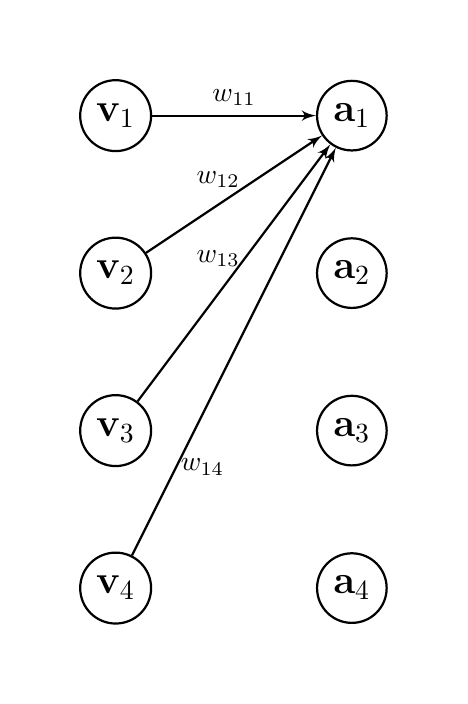
\begin{tikzpicture}[>=latex',thick]

      % nodes to add some white space
      \node [name=upper_left] at (-1, 1) {};
      \node [name=upper_right] at (4, 1) {};
      \node [name=lower_left] at (-1, -7) {};
      \node [name=lower_right] at (4, -7) {};

      % layer 1 
      \node [draw=black, circle, minimum size=25pt, name=l11] at (0, 0) {\Large{$\textbf{v}_1$}};
      \node [draw=black, circle, minimum size=25pt, name=l12] at (0, -2) {\Large{$\textbf{v}_2$}};
      \node [draw=black, circle, minimum size=25pt, name=l13] at (0, -4) {\Large{$\textbf{v}_3$}};
      \node [draw=black, circle, minimum size=25pt, name=l14] at (0, -6) {\Large{$\textbf{v}_4$}};
      % layer 2 
      \node [draw=black, circle, minimum size=25pt, name=l21] at (3, 0) {\Large{$\textbf{a}_1$}};
      \node [draw=black, circle, minimum size=25pt, name=l22] at (3, -2) {\Large{$\textbf{a}_2$}};
      \node [draw=black, circle, minimum size=25pt, name=l23] at (3, -4) {\Large{$\textbf{a}_3$}};
      \node [draw=black, circle, minimum size=25pt, name=l24] at (3, -6) {\Large{$\textbf{a}_4$}};

      % connections
      \draw [->] (l11) -- node [above] {$w_{11}$} (l21);
      \draw [->] (l12) -- node [above, yshift=-0.05cm, xshift=-0.2cm] {$w_{12}$} (l21);
      \draw [->] (l13) -- node [above, xshift=-0.2cm, yshift=-0.05cm] {$w_{13}$} (l21);
      \draw [->] (l14) -- node [above, xshift=-0.4cm, yshift=-1.7cm] {$w_{14}$} (l21);




    \end{tikzpicture}
\end{document}
